%%%%%%%%%%%%%%%%%%%%%%%%%%%%%
%Since : Jan/29/2009
%Update: <Mar/13/2013>
% -*- coding: iso-2022-jp -*-
%%%%%%%%%%%%%%%%%%%%%%%%%%%%%

\chapter{ネットワーク基礎演習2}
\section{目的}

私たちは、日頃なにげなくパソコンや携帯電話でウェブページを閲覧している。
ウェブページはパソコンや携帯電話がネットワークにつながっていないとみることができない。
つまり、みているウェブページのデータはパソコンや携帯電話上には無く、ネットワークを介して自分のパソコンや携帯電話にデータをダウンロードし見ているのである。では、ウェブペー
ジのデータはどこにあるのか。実はウェブページのデータはネットワーク上に存在する、ウェ
ブサーバと呼ばれるコンピュータに入っている。ウェブページを閲覧するためにはウェブサー
バにアクセスし、ウェブページのデータをそこからダウンロードしなければならない。ま
た、ウェブページを公開するためにはウェブサーバにウェブページのデータをアップロー
ドしなければならない。そのようなデータの流れを\figref{fig:server}に示す。
このようなデータの流れは他のサーバでも基本的には同じものである。本実験では,
ウェブページをクライアント上で作り、ウェブサーバに転送し、それをブラウザで閲覧す
ることでファイル転送の仕方、サーバクライアントの関係を学ぶ。さらに、サーバに直接入り、そこでウェブページを更新することで、コンピュータを遠隔操作することを学ぶ。

\begin{figure}[htbp]
\begin{center}
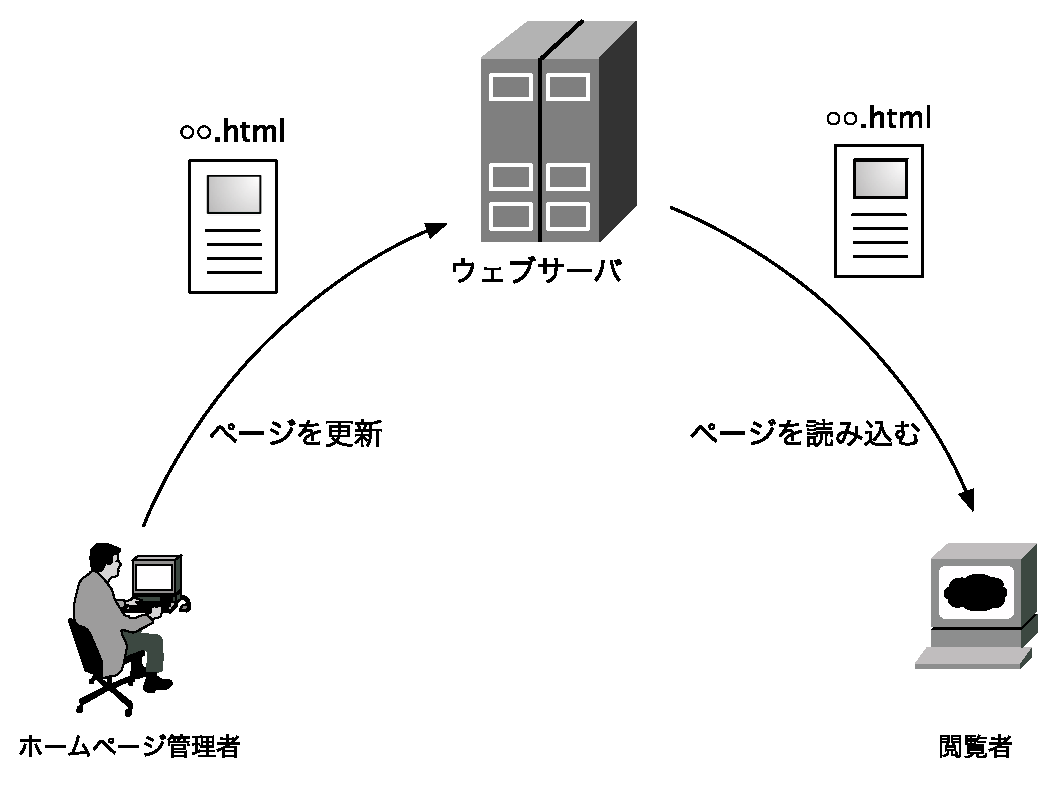
\includegraphics[width=0.8\linewidth]{server.eps}
\caption{ウェブサーバとホームページのデータの流れ。ホームページを管理者が作成し,
    ウェブサーバにそのデータをアップロードする。そのアップされたウェブページのデータ
    を閲覧するクライアントが自分のコンピュータにデータをダウンロードして見る。}
\label{fig:server}
\end{center}
\end{figure}


\section{実験用ウェブサーバ}
実験室には実験用ウェブサーバを設置している。ウェブサーバの名前はcpjwebという名前
になっている。ウェブサーバにはユーザがウェブページを作れるよう設定してある。ユー
ザがウェブページを公開する場合には、cpjwebのホームディレクトリ下の
``public\_html'' にウェブページのデータを保存すればよい。ウェブページのURLは
``http://cpjweb.center.tsuyama-ct.ac.jp/\~{}c-○○○/''である。ここでは、まず,
自分のウェブページが存在することを確認する。

\paragraph{演習}
\begin{enumerate}
\item \figref{fig:browser-icon}の矢印で示すアイコンをクリックし、ブラウザを立ち
      上げる。
\item http://cpjweb.center.tsuyama-ct.ac.jp/\~{}c-○○○/を開く。
\item 開いたら``test''と表示されることを確認する。
\end{enumerate}

\begin{figure}[htbp]
\begin{center}

\includegraphics[width=0.5\linewidth]{browser-icon.eps}
\caption{ブラウザのアイコン}
\label{fig:browser-icon}
\end{center}
\end{figure}

\section{ウェブページ作成}

まず自己紹介ページを作成する。本実験では、UNIX、Linuxでよく用いられる``Emacs''と
いうテキストエディタを用い、ウェブページを作成する。

\paragraph{演習}
\begin{enumerate}
\item ターミナルで``emacs index.html\&''と入力し実行する。実行すると、
      index.htmlという名前のファイルが何もない状態で開かれる(\figref{fig:emacs})。
\item Emacsで実験書にのっているウェブページのソースコードを入力し、ウェブページを作る。
\item 作成できたら保存する。保存の方法は、Controlとxを同時に打ち、次にControlとs
      を同時に打つと保存される。
\item 保存ができたら、Emacsを終了する。終了の方法は、Controlとxを同時に打ち、次に
      Controlとcを同時に打つと終了する。
\item Emacs終了したらブラウザで問題なく表示できるか確かめる。確かめる場合は,
      ``firefox index.html\&''と入力してEnterキーを押す。
\item 自己紹介ページがうまく表示できない場合は、1からやり直し、ウェブページのソー
      スコードをきちんと入力したか確認する。
\end{enumerate}

\begin{figure}[htbp]
\begin{center}
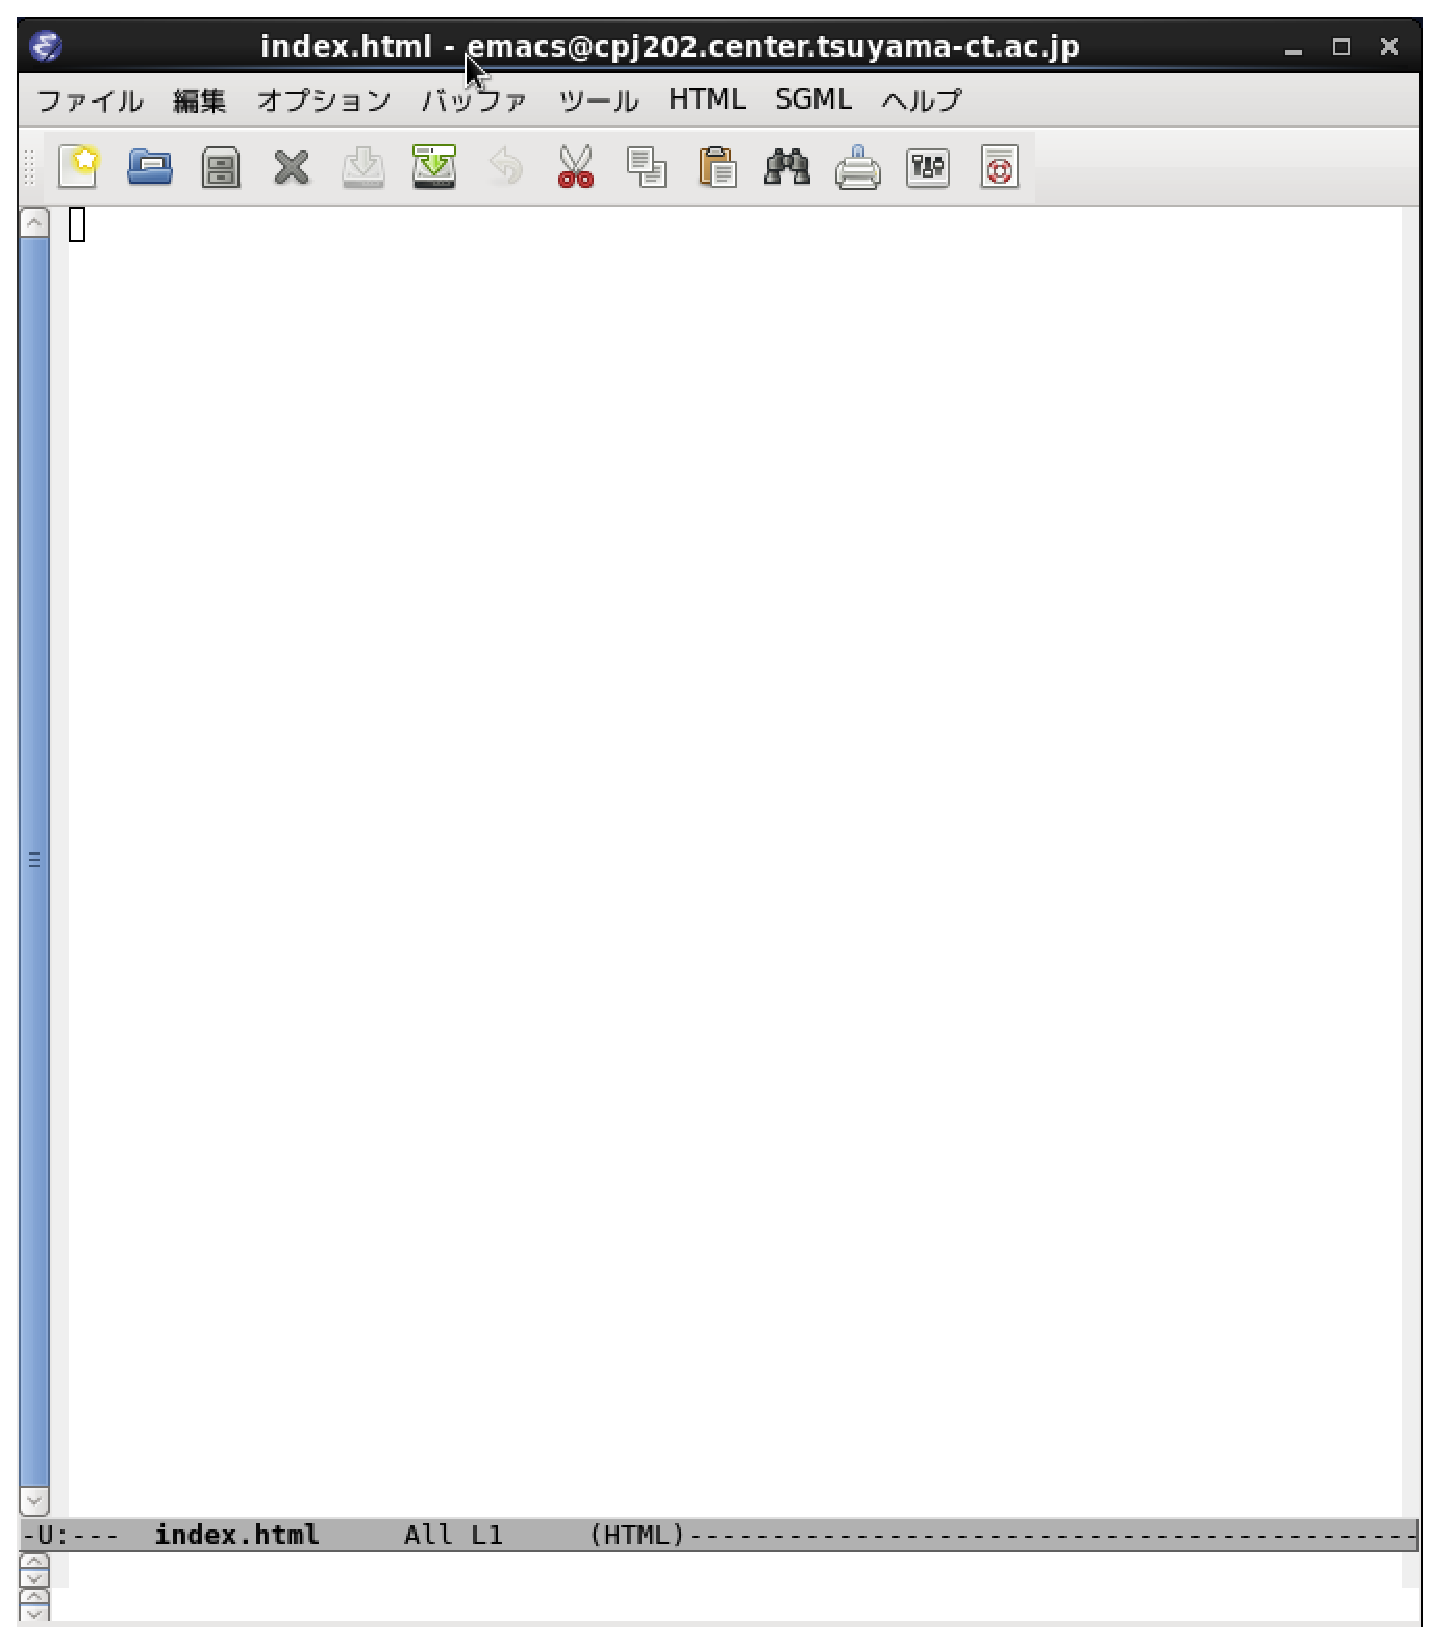
\includegraphics[width=0.5\linewidth]{emacs.eps}
\caption{emacs}
\label{fig:emacs}
\end{center}
\end{figure}

\begin{figure}[htbp]
\begin{center}
{\small リスト2.1: ウェブページのソースコード}
{\small
\begin{verbatim}
<html lang="ja">
    <head>
        <meta http-equiv="content-type" content="text/html; charset=">
        <title>Resume</title>
        <style type="text/css">
            <!--
                h1{
                    border-left: #0000ff 10px solid;
                    border-bottom: #0000ff 4px solid;
                }
                h2{
                    border-bottom: #0000ff 1px solid;
                }
            -->
        </style>
    </head>
    <body>
        <h1>Resume</h1>
        <h2>Name</h2>
            ○○ △△
        <h2>affiliation</h2>
            Department of Computer and Information Engineering,
    </body>
</html>
\end{verbatim}
}
\end{center}
\end{figure}

\section{sftp}
ウェブページを公開するためには、データをウェブサーバに送らなければならない。サー
バにデータを送るために``sftp''を用いる。``sftp''はコンピュータ間でファイルをやり
とりするためによく用いられる。なぜならばsftpは、データのやりとりが暗号化されてお
り、セキュアであるからである。ここでは、sftpを用いてウェブページのデータをウェブ
サーバに送り、ウェブページを公開する。

\paragraph{演習}
\begin{enumerate}
\item ターミナルに``sftp c-○○○@cpjweb.center.tsuyama-ct.ac.jp''と入力してEnterキーを押す。
\item 実行すると接続が開始される。相手のコンピュータに初めて接続するときは、\figref{fig:ssh1}の
      ような質問が表示される。``(yes/no)?''というメッセージの後に``yes/no''と入力してEnter
      キーを押す。
\item 正しく接続できるとパスワードをたずねてくるので、パスワードを入力してEnterキーを押す。この際、パスワードは表示されない(アスタリスクも表示されない)。
\item ログインに失敗すると、``permission denied、please try again''と表示され,
      再びパスワードを入力する。
\item ログインに成功すると、``sftp$>$''のように表示される。sftpで接続している最中は``sftp$>$''
      がコマンドプロンプトになるので、この後に続けてコマンドを入力する。
\end{enumerate}

\begin{figure}[htbp]
\begin{center}
\fbox{
\includegraphics[width=0.8\linewidth]{ssh1.eps}
}
\caption{sftp接続確認画面}
\label{fig:ssh1}
\end{center}
\end{figure}

\subsection{cd}
sftp でログインした際の最初のカレントディレクトリは、コンピュータの設定によりま
ちまちである。cpjwebの場合は各自のホームディレクトリ(/home/c-○○○)に設定されて
いる。ウェブサーバcpjwebでは、各ユーザのホームディレクトリ下の``public\_html''に
ウェブページのデータを置くことで、ウェブページが公開されるよう設定されている。
そこにデータを置くため、カレントディレクトリを変更しなければならない。そのために``cd''
というコマンドを使用する。

\paragraph{演習}
\begin{enumerate}
\item コマンドプロンプトに続いて``cd  public\_html''と入力してEnterキーを押す。
\item コマンドプロンプトに続いて、``pwd''と入力してEnter キーを押す。カレントディレ
      クトリが``/home/c-○○○/public\_html''となっていることを確認する。カレントディレクトリ
      が異なる場合は1の作業を再度行う。
\item コマンドプロンプトに続いて``ls''と入力してEnter キーを押す。index.htmlファ
      イルがあるか確認する。
\end{enumerate}

\subsection{lcd}
ローカル・コンピュータのカレントディレクトリを変更するには、``lcd''というコマン
ドを使用する。

\paragraph{演習}
\begin{enumerate}
\item コマンドプロンプトに続いて``lcd  /homes/c-○○○''と入力する。
\item 異なるディレクトリに変更してしまった場合や、変更に失敗
      した場合は1の作業を再度行う。
\end{enumerate}

以上の作業により、リモート側のディレクトリは``/homes/c-○○○/public\_html''に設定され、ロー
カル側のディレクトリは``/homes/c-○○○''に設定された。


\subsection{put}
リモート・コンピュータへローカル・コンピュータからファイルを送るには、``put''
というコマンドを使用する。

\paragraph{演習}
\begin{enumerate}
\item コマンドプロンプトに続いて``put index.html''と入力してEnterキーを押す。
\item 正しく入力できたときは、\figref{fig:put}に示すように、転送速度や転送にかかった時間が表示
されたあと、コマンドプロンプトに戻る。失敗した場合は、ファイルが存在しないな
どのメッセージが表示される。失敗しているときはもう一度転送を試みる。
\end{enumerate}

\begin{figure}[htbp]
\begin{center}
\fbox{

\includegraphics[width=0.8\linewidth]{put.eps}
}
\caption{putの実行例}
\label{fig:put}
\end{center}
\end{figure}

\subsection{exit}
sftpの接続を切断するには``exit''というコマンドを使用する。

\paragraph{演習}
\begin{enumerate}
\item コマンドプロンプトに続いて、``exit''と入力してEnterキーを押す。
\item 通常のコマンドプロンプトに戻ったことを確認する。戻っていなければ、1の作業を
      再度行う。
\end{enumerate}


\section{コンピュータの遠隔操作}
昔はコンピュータが大型(教室と同じかもっと大きかった)で高価であったため、それ
ぞれの企業や学校で1台という状況であった。そこで、端末(Terminal)と呼ばれるキー
ボードとモニターだけを持つ装置をいくつか設置して、これらとホストコンピュータとを
専用線で接続して、何人かで共有して利用していた。現在に置き
換えると、1 台のパソコンに複数のキーボードとモニターを接続した状態である。ホスト
コンピュータにはマルチタスクのOSが備えられており、それぞれの端末から入力される
タスクを並行に実行していた。一般に各回線はホストコンピュータに直接接続する必要が
あるが、その長さは数十kmにも及ぶことがあった。

コンピュータの小型化・低価格化により、高価なホストコンピュータを1台だけ購入す
るよりも、安価で小型のコンピュータ(パソコンなど)をいくつか購入して、それぞれに
独立して処理を行わせるほうがコストも低く、仕事の効率もよくなった。しかし、大規模
な計算を行わせたり、利用者の間で大量のデータを共有したりするときには、高性能で大
規模なメモリやディスクを備えたコンピュータが必要になる。そして、LANやインター
ネットに代表されるネットワークの普及により、ネットワークを利用して以前の端末と同
じように、遠隔のコンピュータに接続して、操作するためのソフトウェアが必要になった。
端末の機能を実現するソフトウェアを端末エミュレータ(Terminal Emulator)と呼び,
ネットワークを介して遠隔のコンピュータ(リモート・コンピュータ)と接続して、コマ
ンドや実行結果の送受信を行う技術をTELNET と呼ぶ。UNIXでは端末エミュレータと
TELNETの機能により、1つのコンピュータに複数の利用者が同時にログインして操作を
行うことも、ネットワークを介して1台のコンピュータから複数のコンピュータにログイ
ンし、それぞれに処理を行わせることが可能である。この様子を図2に示す。各自、自分
が使用しているコンピュータで何らかの作業をしながら、他のコンピュータにログインし
て操作したり、プログラムを実行することが可能である。特に長い計算をするプログラム
であれば、先週に学習したように、バックグラウンドで実行した後でログアウトしておき,
後日に再びログインして結果を見ればよい。


\section{ssh}

SSH(Secure Shell)は、ローカル・コンピュータとリモート・コンピュータの間で送受
信される情報に暗号化を施しながら、TELNETと同様の機能を実現する技術である。TELNET
は暗号化されていないため、現在はSSHを用いることが主流となっている。実験
ではSSHを使用して、ウェブサーバcpjwebにコンピュータに接続する。

\paragraph{演習}
\begin{enumerate}
\item ターミナルに、``ssh -l ユーザ名 cpjweb.center.tsuyama-ct.ac.jp''と入力して
      Enterキーを押す。
\item \figref{fig:ssh2}のようにパスワードを入力するようなメッセージが表示されるので、現在のコン
      ピュータにログインしたときと同じパスワードを入力する。
\item パスワードが正しくないときは、再びパスワードを質問される。何度か失敗すると接
      続を切られてしまうので、再度コマンドを入力して接続を試みる。
\item 正しく接続できたときは、これまでと同じようにコマンドプロンプトが表示されるが,
      ホスト名を示す部分がcpjwebに変更されている。
\item ログインに成功したら、コマンドプロンプトに続いて``who''と入力してEnterキーを
      押す。このコマンドはコンピュータにログインしているユーザを表示するものである。
      実験受けている学生が表示されるか確認する。
\end{enumerate}

\begin{figure}[htbp]
\begin{center}
\fbox{

\includegraphics[width=0.8\linewidth]{ssh2.eps}
}
\caption{SSHの使用例}
\label{fig:ssh2}
\end{center}
\end{figure}

\section{ウェブサーバ上でのホームページの更新}
これまでは、ウェブページをクライアント側で編集し、サーバにアップロードしてウェブ
ページを更新してきた。ネットワークの世界では、サーバに直接入りファイルを書き換え
る作業を行うことも良くある。その練習のため、ウェブサーバcpjwebにsshでリモートア
クセスし、ウェブページを更新する。

\paragraph{演習}
\begin{enumerate}
\item cpjwebに入ったまま次の作業を行う。
\item cdコマンドを用いウェブページのデータが保存されているpublic\_htmlに移動する。
\item ``emacs index.html''と入力し実行し、index.htmlをEmacsで開く。
\item index.htmlにDepartment...の行末で改行し、新たな行に``Tsuyama National
      College of Technology''を追加し、保存してEmacsを終了する。Emacsを終了するに
      は、Controlとxを同時に押し、次にControlとcを同時に押すことで終了する。
\item ブラウザで情報が更新されたか確認する。
\item 確認が終わったら``exit''と入力して実行することで、cpjwebからログアウトする。
\end{enumerate}


\section{演習問題}

\begin{enumerate}

\item ウェブページを作成し公開するまでの流れを説明せよ。

\item sftpを使用して、cpjwebというコンピュータに接続するときに使用するコマンドを
      書け。

\item sftp で離れたコンピュータに接続しているとき、そのリモートコンピュータでのカレ
      ントディレクトリを``/homes/data''に変更するために使用するコマンドを書け。

\item sftp で離れたコンピュータに接続しているとき、ローカルコンピュータでのカレント
      ディレクトリを``/homes/data''に変更するために使用するコマンドを書け。

\item SSHでウェブサーバcpjwebに入るためのコマンドを書け。

\item リモートでコンピュータを操作する利点は何か。

\end{enumerate}
